%input{symbols}

\section{Projecting damages of individual actions}
Given all the relevant factors in a damage calculation, it is possible to express the average damage of an ability or action.
In this section, we'll derive expressions that give the average damage, or projected damage, of various actions a ret can perform.
%Now that we have detailed BCC's combat system and its facets relevant to a ret paladin's damage output, we may now turn to the task of quantifying the projected damage of various actions a ret paladin can take.
%It is of interest to be able to compare projected damage outputs of various individual actions and rotations without having to simulate entire gear sets.
%Unfortunately, many aspects of a paladin's gear directly affect the relative effectiveness of different actions and rotations.
%These effects are often small, but can be significant.
%For example:
%\begin{itemize}
%	\item the paladin's Expertise affects the chance for their attacks to be dodged. When the dodge chance is lower, swing actions that involve many segments of damage being chained together increase in relative value to ``simpler'' swings, as a dodge breaking the damage chain is less likely to occur.
%	\item the Libram of Avengement crit buff is \emph{relatively} more effective in gear sets that have low amounts of Critical Strike Chance, and therefore rotations that provide the ability to use judgement on cooldown rise in \emph{relative} value more for lower crit gear sets (though the effects are almost certainly very small)
%\end{itemize}
%It is desirable to reduce gear sets to the lowest amount of input variables possible such that these effects can be accounted for.

\subsection{Relative damages}
When figuring out what the best option for a ret's rotation, it is not always strictly necessary to include the full damage calculation.
Let us consider the case of evaluating how riding blood and command for a swing compare to one another.
Both benefit equally from any global modifiers to a paladin's damage, e.g. $2~\%$ from the Improved Sanctity Aura talent.
They also benefit equally from the $6~\%$ damage modifier to damage dealt with two-handed weapons from the Two-Handed Weapon Specialisation talent.
We therefore do not need to include these damage scaling factors when comparing riding SoC to SoB.

An example of a relevant damage factor is Sanctity Aura itself, which increases all holy damage done by $10~\%$.
If swinging SoB and SoC have a different average amounts of holy damage (spoiler: they do) then sanctity aura affects the relative worth of riding SoC vs SoB.
In this section, we will only be analysing the following actions as independent events:
\begin{itemize}
	\item autoattacks and windfury attacks
	\item seal damage, including twists
	\item crusader strike
\end{itemize}
The statistics affecting the relative damage of each of these actions are:
\begin{itemize}
	\item total attack AP, given the differing normalisations of CS and the other actions, and the bonus AP scaling on windfury attacks
	\item dodge chance
	\item armor penetration and boss armor
	\item crit strike chance (because it is correlated with dodges in autoattacks but not for seals)
	\item the base weapon speed
	\item the mean base weapon damage
\end{itemize}
With each of these variables, it is possible to evaluate the relative projected damages of each action entirely.

\subsection{Physical and Holy global scale factors}
We now define the following global scaling factors for physical and holy damage, i.e. scale factors that will apply to \emph{every instance of physical or holy damage} that is not negated by a dodge.
For physical damage:
\begin{equation}
	\fphys = 1 - \frac{\armor - \armpen + 1}{467.5 \lvl -22167.5}
\end{equation}
where \armor is the target armor, \armpen the ret's armor penetration, and \lvl the target level.
\noindent
For holy damage:
\begin{equation}
	\fholy = 0.94 \times 1.1 = 1.034
\end{equation}
where the first term is the average reduction from partial resists, and the latter term the damage bonus to holy abilities from Sanctity Aura.

\subsection{Units of damage}
Seal of Blood, Seal of Command, and Crusader Strike are all evaluated in terms of a percentage of the paladin's weapon damage.
The average weapon damage of a paladin's basic autoattack is therefore a useful metric to start with.
We first define the average weapon damage as the damage that occurs when a weapon rolls a median value on its damage range, and is a regular hit (i.e. not a crit, or a glancing blow) that is not negated (through a miss or dodge).
\begin{equation}
	\dave = \left( \bar{\wdam} + \frac{x\ws}{14} \right)
\end{equation}
where $\bar{\wdam}$ is the median damage on the weapon's damage range, $x$ is the paladin's attack power, and \ws is the paladin's weapon speed.
We note that this is not applicable to CS, which has a different scaling with attack power, but this value can be used for autoattack and seal damages.

\subsection{Correlation of attacks}
Let us first consider the damage \dauto of so-called ``white hits'', meaning a simple autoattack.
The \dave figure is useful because it allows for all results of an attack table roll to be expressed in some multiple of \dave:
\begin{equation}
	\dauto = \fphys \dave \sum_n p_{\mathrm{n}} f_{\mathrm{n}}
\end{equation}
where the sum is over the $n$ possible outcomes for the attack roll that are left on the table (e.g. crit, dodge \ldots), with each scenario having a probability to occur $p_{\mathrm{n}}$, and a damage scaling factor for its outcome of $f_{\mathrm{n}}$ (e.g. $\fcrit = 2.06$ with an activated Relentless Earthstorm Diamond meta-gem).
Giving these outcomes explicitly, we arrive at the expression:
\begin{equation}
	\dauto = \fphys \dave (\pdodge \fdodge + \pglance \fglance + \pcrit \fcrit + \phit \fhit)
\end{equation}
where \pdodge and \fdodge are the probability and damage scaling of a dodge, and the other outcomes correspond to glances, crits, and regular hits. 

This expression can be simplified first by giving $\fdodge = 0$ (as dodges are negated entirely), \fhit as simply 1, and then describing \phit as the difference of 1 and the probability of all other attack outcomes (given hit expands to take up the remainder of the attack table), or
\begin{equation}
	\phit = 1 - \pglance - \pdodge - \pcrit
\end{equation}
The expression for the projected autoattack damage then becomes:
\begin{equation}
	\dauto = \fphys \dave (\pglance \fglance + \pcrit \fcrit + (1 - \pdodge - \pglance - \pcrit))
\end{equation}
The above expression projects the expected average damage from a simple autoattack, including outcomes where the attack is negated entirely from a dodge.

We note, however, that many parts of a paladin's damage output \emph{proc subsequent instances of damage that are conditional on the result of the initial part}.
In other words, a dodged attack cannot proc anything else.
If the outcome for negated attacks is included in our standard damage unit, then damage chains get messily correlated in ways that make the calculations very difficult.

Take windfury as an example.
It's not possible to say that the expected damage under windfury is therefore just an extra $20\%$ of \dauto because the expression for \dauto includes the chance for the attacks to be dodged - and if the first attack is dodged, the windfury attack never occurs.

\subsection{Fixing this problem}
We therefore want to derive an expression for the projected physical damage of an attack \emph{independently of the chance for it to be dodged}.
This is complicated by \pdodge affecting the relative magnitudes of \phit, \pglance, and \pcrit arising from the use of a single-roll attack table.
Therefore even when deriving an expression that describes only the case when the attack is \emph{not dodged}, we still expect to see \pdodge as a relevant factor.

We therefore define \dphys as the \emph{average damage from an attack that connects with the enemy}, i.e. is not dodged.
\begin{equation}
	\dphys = \fphys \dave \frac{(\pglance \fglance + \pcrit \fcrit + (1 - \pglance - \pdodge - \pcrit)}{1 - \pdodge}
\end{equation}

Note that despite the presence of two \pdodge terms, the average damage is projected \emph{only onto scenarios in which the attack connects and is not negated}.
We also see the well-established concept of a maximum limit below 1.0 on critical hit probability, or ``crit cap'' manifest in this equation, in the form of the necessary inequality:
\begin{equation}
	\pcrit \leq (1-\pglance - \pdodge)
\end{equation}
As glance and dodge have higher \emph{precedence} than crit, it can never push them off the attack table.
As such, any crit probability above $1 - \pglance - \pdodge$ will be ignored.

\subsubsection{An Example Calculation with Windfury Attack}
To see why this formulation is useful, let us now derive the projected damage in the case of a naked windfury swing in these terms.
%The typical raiding values for the above correspond to $\pglance = 0.24$, $\fglance = 0.75$, $\fcrit = 2.06$, with a probability of proccing Windfury $\pwf = 0.2$.

To be exact, we must consider that the windfury attack has an amount of bonus attack power, that depends on the rank of the Windfury Totem and the Shaman's talents.
If the ret paladin's attack power is $x$ and the bonus attack power on the Windfury Attack is $y$, the $\dave(\mathrm{wf})$ on the Windfury attack can be expressed as a fraction of the autoattack's \dave as:
\begin{equation*}
	\begin{aligned}
		\frac{\dave(\mathrm{wf})}{\dave} &= \frac{\wdamave + \frac{(x+y)\ws}{14}}{\bar{\wdam} + \frac{x\ws}{14}} \\
		&= \frac{\wdamave + \frac{\ws x + \ws y}{14}}{\wdamave + \frac{\ws x}{14}}
	\end{aligned}
\end{equation*}
We can therefore define a scale factor
\begin{equation}
	\fwf = \frac{\wdamave + \frac{\ws x + \ws y}{14}}{\wdamave + \frac{\ws x}{14}}
\end{equation}
which is the relative damage of a Windfury hit (with bonus Windfury attack power $y$, a paladin's attack power $x$, and a weapon speed \ws) to a normal autoattack hit.

The projected damage of a naked hit with Windfury active and a non-zero \pdodge is then:
\begin{equation*}
	\begin{aligned}
		d_\mathrm{wf} &= (1 - \pdodge) \dphys + (1 - \pdodge)^2 \pwf \fwf \dphys\\
				&= \dphys\left(1 - \pdodge + \pwf\fwf(1 -\pdodge)^2\right) \\
	\end{aligned}
\end{equation*}
This equation is expressed entirely in terms of our \dphys variable, the dodge chance, and the Windfury proc chance and damage scaling factor.
With this equation, you can plug in some values for the ret's stats and determine the relative benefit of swinging with windfury up over not having it.


\subsubsection{Quick aside: single attack table weirdness}
This all has some slightly counter-intuitive effects:
\begin{itemize}
	\item Low Expertise gear sets do slightly more damage on average when they hit, do less overall damage on average from being dodged more, and benefit disproportionately from Critical Strike Chance.
	\item Low Expertise gear sets do slightly less damage on average when they hit, do more overall damage on average from being dodged less, and benefit slightly less from Critical Strike Chance than low Expertise gear sets.
\end{itemize}
Ultimately because of the construction of the single-roll attack table, this makes sense.
Crits are independent of negations like miss or dodge, so regardless of your dodge chance you will crit on average the same number of swings with a given crit chance (provided you are not near the crit cap).

We provide in \tabref{tab:wfautos} some example calculations of windfury damage for three different dodge chance scenarios, in each calculating the projected damage of a set with $10\%$ crit and one with $40\%$ crit.
For each scenario, we can see that the relative benefit of moving to a higher crit value changes as a function of the dodge chance, again due to quirks in the single-roll attack table.

\begin{table}[htb]
	\centering
%	\title{Windfury attacks w.r.t. crit and dodge chance}
	\begin{tabular}{ r | r | r | r | r | l }
		  \multicolumn{1}{c|}{}  & Dodge Chance & Crit Chance & Projected \dphys & Projected \dwf & Crit Benefit \\
		\hline \hline
		\multirow{2}{*}{Scenario 1}	 &	\multirow{2}{*}{0.065} & 0.1 & $1.049~\dave$ & $1.164~\dave$ & \multirow{2}{*}{1.324} \\
					&  & 0.4 & $1.389~\dave$ & $1.542~\dave$ & \\
		\hline
		
		\multirow{2}{*}{Scenario 2}	 &	\multirow{2}{*}{0.0325} & 0.1 & $1.048~\dave$ & $1.210~\dave$ & \multirow{2}{*}{1.314} \\
		&  & 0.4 & $1.377~\dave$ & $1.589~\dave$ & \\
		\hline
		
		\multirow{2}{*}{Scenario 3}	 &	\multirow{2}{*}{0.0} & 0.1 & $1.046~\dave$ & $1.255~\dave$ & \multirow{2}{*}{1.304} \\
		&  & 0.4 & $1.364~\dave$ & $1.637~\dave$ & \\
		\hline
		
	\end{tabular}
	\caption{How dodge chance interacts with critical strike chance.
		\dave encodes all information on the user's weapon and Attack Power, so these results hold across all gear sets.
	The projected \dphys is the average damage of a connecting attack i.e. an attack that is not dodged.
	The projected \dwf is the average damage of a swing under windfury, including the chances for the attacks to be dodged.}		
	\label{tab:wfautos}
\end{table}

Somewhat frustratingly, we cannot naively say that e.g. the P2 BiS Blood-Elf scenario with 24 Expertise and $\pdodge = 0.005$ is better than a no-Expertise scenario with $\pdodge = 0.065$ by a factor of $1.193005/1.109845 \approx 1.075$.
We can only say how the relative levels of Expertise compare \emph{as a function of Critical Strike Chance}, even if the effect is marginal in most cases.

This is also why, if you somehow manage to hit a rogue with Evasion up, it will have a very high chance of being a crit, as all the lower precedence regular hits have been pushed off the table.
In that very fringe case, you don't benefit much from a high value of critical strike chance; even low crit chance gear sets will crit if they hit.

\subsection{Seal of Command swing - no windfury}
We now turn to projecting the damage of swinging with Seal of Command active, without windfury.
We no longer have to worry about the single-rolled attack table given that special attacks use an independent roll to determine if the attack connects.
We do, on the other hand, now have to worry about the differences between holy and physical damage to properly quantify the projected damage.

Using the units of damage we have arrived at previously, the damage of a SoC proc on a regular hit is simply:
\begin{equation}
	\dsocproc(\mathrm{hit}) = \fholy \left( 0.7  \dave + \fspell (\dspell + \bspell) \right)
\end{equation}
where \fspell if the SoC spellpower coefficient of 0.2, \dspell is the ret's spellpower, and \bspell is the bonus spell power to abilities cast on the target (from abilities like JotC).
When we include the chance for regular hits and crits (and because a successful seal attack can \emph{only} hit or crit):
\begin{equation}
	\dsocproc = \dsocproc(\mathrm{hit}) \times ( \pcrit \dcrit + 1 - \pcrit)
\end{equation}
AS a reminder, the proc chance for SoC is determined by the base weapon speed \ws:
\begin{equation}
	\psoc = \frac{7 \ws}{60}
\end{equation}
When we combine this with the auto that must connect to proc the SoC, taking into account the relevant dodge chances, we find the following damage projection for a swing with SoC active:
\begin{equation*}
	\begin{aligned}
		\dsocswing =&~ (1-\pdodge) \left( \dphys + (1 - \pdodge) \psoc \dsocproc \right) \\
%		=& \dphys - \pdodge \dphys + (1-\pdodge) \psoc \dsocproc - \pdodge(1 - \pdodge) \psoc \dsocproc\\
		=&~ (1 - \pdodge) \dphys + (1 - \pdodge)^2 \psoc \dsocproc\\
	\end{aligned}
\end{equation*}

\subsection{Seal of Command swing - with windfury}
The SoC ICD means that only one melee hit can proc SoC.
If the first hit procs SoC, the second cannot, and vice-versa.
We also find two possible damage chains that can occur:
\begin{enumerate}
	\item The initial melee procs \emph{both} windfury attack and SoC.
	\item The initial melee procs \emph{only} windfury attack, which subsequently procs SoC.
\end{enumerate}
Each case results in a different number of dodge checks to be passed.
In the first case the projected damage is:
\begin{equation*}
	\begin{aligned}
		\dsocswing (1) =&~ (1-\pdodge) \dphys + (1-\pdodge)^2 \psoc\dsocproc + (1-\pdodge)^2 \pwf \fwf \dphys\\
	\end{aligned}
\end{equation*}
In the second case the projected damage is:
\begin{equation*}
	\begin{aligned}
		\dsocswing (2) =&~ (1-\pdodge) \dphys + (1-\pdodge)^2 \pwf \fwf \dphys + \pwf (1-\pdodge)^3 \psoc\dsocproc\\
	\end{aligned}
\end{equation*}
These cases are mutually exclusive. Projecting over them both we find:
\begin{equation*}
	\begin{aligned}
		\dsocswing =&~ (1-\pdodge) \dphys + (1-\pdodge)^2 \pwf \fwf \dphys \\
		&+ (1-\pdodge)^2 \psoc\dsocproc \\
		&+ (1-\psoc)(1-\pdodge)^3 \pwf \psoc \dsocproc \\
		=&~  \dphys(1 - \pdodge + \pwf\fwf(1 -\pdodge)^2) \\
		&+ (1-\pdodge)^2 (1+\pwf(1-\pdodge)(1-\psoc)) \psoc\dsocproc 
	\end{aligned}
\end{equation*}
Note that the physical damage reduces down to the same result as for a naked swing under windfury; simply put, your basic attacks don't care what seal you have active, they hit all the same. We show the SoC under windfury as a function of the weapon speed in Figure \ref{fig:soc_wf} - it is very slightly nonlinear, with the proc chance increasing under windfury less at higher weapon speeds.

\begin{figure}[ht] 
	\centering 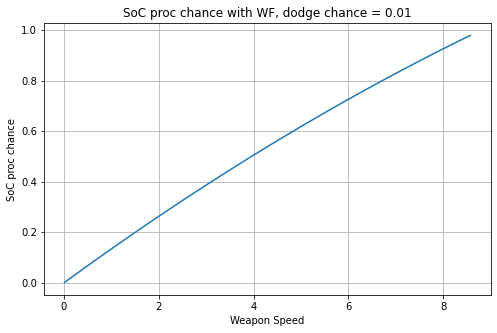
\includegraphics[width=0.84\columnwidth]{figs/wf_soc_1.png}
	\caption{SoC proc chance under windfury as a function of weapon speed, \pdodge = 0.01}
	\label{fig:soc_wf}
\end{figure}

\newpage
\subsection{Seal of Blood swing - no windfury}
Seal of Blood is a simpler ability to forecast because it has no internal ICD, meaning that there is no correlation between the SoB procs, it has no spellpower coefficient, and the proc is guaranteed.
The proc damage on a regular hit is therefore identical to the physical damage, times the $35~\%$ weapon damage scaling, and the global holy damage factor:
\begin{equation}
		\dsobproc(\mathrm{hit}) = \fholy 0.35  \dave
\end{equation}
and the corresponding damage accounting for crit chance is
\begin{equation}
	\dsobproc = \dsobproc(\mathrm{hit}) \times (\pcrit \dcrit + 1 - \pcrit)
\end{equation}
The damage for a SoB swing without windfury is therefore:
\begin{equation}
	\dsobswing = (1 - \pdodge) \dphys + (1-\pdodge)^2 \dsobproc
\end{equation}

\subsection{Seal of Blood swing - with windfury}
There is only one damage sequence for a SoB hit under windfury: the initial melee procs a SoB that must survive the standard two dodge rolls.
The windfury attack if procced must also survive two dodge rolls, and its SoB proc must survive three dodge rolls.
The damage projection for the full swing is therefore:
\begin{equation*}
	\begin{aligned}
		\dsobswing =&~ (1 - \pdodge) \dphys + (1-\pdodge)^2 \dsobproc \\
		&+ \pwf \left( (1-\pdodge)^2 \fwf \dphys + (1-\pdodge)^3 \dsobproc \right)
	\end{aligned}
\end{equation*}


%%%%%%%%%%%%%%%%%%%%%%%%%%%%%%%%%%%%%%%%%%%%%%%%%%%%%%%%%%%%%%%%%%%%%%%%
\subsection{Twist attempt - no windfury}
We now combine the information from swinging under blood and command to arrive at the damage projection for a twist attempt.
The damage sequence is as follows:
\begin{itemize}
	\item the initial melee must survive a single dodge roll, proccing a SoB that must survive two dodge rolls
	\item if command is procced, it must survive two dodge rolls, proccing a SoB that must survive three dodge rolls.
\end{itemize}
The expression is then:
\begin{equation*}
	\begin{aligned}
		\dsobswing =&~ (1 - \pdodge) \dphys + (1-\pdodge)^2 \dsobproc \\
		&+  \psoc  \left( (1-\pdodge)^2\dsocproc + (1-\pdodge)^3 \dsobproc \right)
	\end{aligned}
\end{equation*}

\subsection{Twist attempt - with windfury}
Windfury, as in the SoC swing case, introduces two possible chains for the damage procs:
\begin{enumerate}
	\item The initial melee procs both wf and SoC.
	\item the initial melee procs wf, which in turn procs SoC.
\end{enumerate}
The damage projection over the first chain is:
\begin{equation*}
	\begin{aligned}
		\dtwist (1) =&~ (1 - \pdodge) \dphys + (1-\pdodge)^2 \dsobproc \\
		&+ \psoc (1-\pdodge)^2 (\dsocproc + (1-\pdodge) \dsobproc) \\
		&+ \pwf (1-\pdodge)^2 (\fwf \dphys + (1-\pdodge)^3 \dsobproc) 
	\end{aligned}
\end{equation*}
while the damage projection over the second chain is:
\begin{equation*}
	\begin{aligned}
		\dtwist (2) =&~ (1 - \pdodge) \dphys + (1-\pdodge)^2 \dsobproc \\
		&+ \pwf (1-\pdodge)^2 (\fwf \dphys + (1-\pdodge)^3 \dsobproc) \\
		&+  \pwf \psoc (1-\pdodge)^3 (\dsocproc + (1-\pdodge) \dsobproc) \\
	\end{aligned}
\end{equation*}
Combining these two mutually exclusive chains, we find the projected damage for a windfury twist attempt:
\begin{equation*}
	\begin{aligned}
		\dtwist =&~ (1 - \pdodge) \dphys + (1-\pdodge)^2 \dsobproc \\
		&+ \psoc (1-\pdodge)^2 \left( \dsocproc + (1-\pdodge) \dsobproc \right) \\
		&+ \psoc\pwf (1-\pdodge)^2 \left(\fwf \dphys + (1-\pdodge) \dsobproc \right) \\
		&+ \pwf (1-\psoc) (1-\pdodge)^2 \left(\fwf \dphys + (1-\pdodge) \dsobproc \right) \\
		&+ \pwf(1-\psoc)(1-\pdodge)^3 \left( \dsocproc + (1-\pdodge) \dsobproc \right) \\
		=&~ (1 - \pdodge) \dphys + (1-\pdodge)^2 \dsobproc \\ 
		&+ (1-\pdodge)^2 \pwf \left( \fwf \dphys + (1 - \pdodge) \dsobproc \right) \\ 
		&+ (1-\pdodge)^2  \left( \psoc + (1-\pdodge)(1-\psoc)\pwf \right) \times \left( \dsocproc + (1-\pdodge)\dsobproc \right)
	\end{aligned}
\end{equation*}


